\documentclass[12pt,letterpaper]{article} %12-point font, US letter size
\usepackage{mathptmx} %Times new roman with math support
\usepackage{fontenc}
\usepackage[english]{babel}

\usepackage{amsmath,amssymb} %math support

%figures
\usepackage[pdftex]{graphicx} 
%\usepackage{epstopdf}

%bibliography
\usepackage{natbib} 
\bibliographystyle{evolution}

%colored hyperlinks
%\usepackage{hyperref}
%\usepackage[all]{hypcap}
%\hypersetup{
%     colorlinks   = true,
%     citecolor    = blue
%}
%\usepackage{color} %for notes to myself

%number pages
\usepackage{fancyhdr}
\pagestyle{fancy}
\pagenumbering{arabic}
\lhead{}
\rhead{\thepage}
%\cfoot{center of the footer!}
\renewcommand{\headrulewidth}{0pt}
%\renewcommand{\footrulewidth}{0pt}
%\fancyfoot[C]{}

%\usepackage{fullpage}
\usepackage{setspace} %double spacing
\usepackage{lineno} %line numbers

\begin{document}

\doublespacing
\linenumbers

%%%%%%%%%%%%%%%%%%%%%%%%%%%%%%%%%%%
%%%%%%%%%%%%%%%%%%%%%%%%%%%%%%%%%%%
\newpage
%\pagestyle{headings}
\setcounter{page}{1}
%\pagenumbering{arabic}
\pagestyle{fancy}

\noindent{\large{\textbf{An evolutionary tipping point in a changing environment}}}%max 50 words
\normalsize

\section*{Abstract} %max 200 words


Populations can persist in directionally changing environments by evolving. Quantitative genetic theory aims to predict critical rates of environmental change beyond which populations go extinct. Here we point out that all current predictions effectively assume the same specific fitness function. This function causes selection on the standing genetic variance of quantitative traits to become increasingly strong as mean trait values depart from their optima. Hence, there is no bound on the rate of evolution and persistence is determined by the critical rate of environmental change at which populations cease to grow. We then show that biologically-reasonable changes to the underlying fitness function can impose a qualitatively different extinction threshold. In particular, inflection points caused by weakening selection create local extrema in the strength of selection and thus in the rate of evolution. These extrema can produce evolutionary tipping points, where long-run population growth rates drop from positive to negative values without ever crossing zero. Generic early-warning signs of tipping points are found to have little power to detect imminent extinction, and require hard-to-gather data. Furthermore, we show how evolutionary tipping points produce evolutionary hysteresis, creating extinction debts. 

%3-6 keywords
\noindent \textit{Keywords:} \textbf{Evolutionary rescue, extinction, fitness function, hysteresis, mathematical model, quantitative genetics}

\newpage
\section*{Introduction}

Many populations currently face gradual directional changes in their environment \citep[reviewed in][]{Davis2005,Parmesan2006,Visser2008,Lavergne2010,Hoffmann2011}.
Those populations with limited dispersal and plasticity can persist only if they evolve fast enough \citep{Lynch1993}.
The maximum rate of environmental change a population can adaptively track -- and demographically tolerate -- %is dubbed the `critical rate of environmental change' \citep{Lynch1991}. The critical rate of environmental change 
has recently received considerable theoretical attention \citep[reviewed in][]{Walters2012,Kopp2013,Alexander2014}. 

Typically these studies follow a quantitative genetic approach \citep[for alternatives see][]{Johansson2008,Bertram2016,Osmond2017}.
They first assume some unimodal mapping from phenotype to absolute fitness (the `fitness function').
Then, for a given rate of change in the trait value that maximizes fitness (the `environmental optimum'), the fitness function is used to derive the rate of evolution in the mean trait value and the expected difference between the mean trait value and the optimum at equilibrium (the `steady-state lag').
The rate of environmental change that produces a steady-state lag resulting in a population mean growth rate (when rare) of zero is dubbed the `critical rate of environmental change' \citep[][]{Lynch1991}.
Critical rates of environmental change are now being estimated and used to predict whether particular species will survive or go extinct in the face of global climate change \citep{Aitken2008,Willi2009,Gienapp2013,Vedder2013}.

To the best of our knowledge, all quantitative genetic theory developed so far implicitly assumes that the maximum rate of environmental change to which a population can adapt is determined by demography (i.e., `selective load' \textit{sensu} \citealt{Lynch1993}, or `demographic constraint' \textit{sensu} \citealt{Gomulkiewicz2009}). 
This assumption results from the shape of the specific fitness functions used.
In particular, Gaussian fitness functions, $W(z)$, are used in models with non-overlapping generations in discrete time \citep{Charlesworth1993c,Burger1995,Burger1997,Burger1999a,Gomulkiewicz2009,Chevin2010,Matuszewski2015,Marshall2016}, while quadratic fitness functions, $r(z)$, are used in models with overlapping generations in continuous time \citep{Pease1989,Lynch1991,Lynch1993,Polechova2009,Aguilee2016}.
These are equivalent given $\log(W)=r$ \citep[][Chapter 1]{Crow1970} and have presumably been chosen for mathematical convenience (e.g., they maintain a normal trait distribution) as well as their ability to approximate -- when near the optimum -- any smooth fitness function imposing stabilizing selection \citep[][]{Lande1976}.
This particular fitness function is therefore a relatively mild assumption under the historical paradigm of weak selection, but it becomes a strong yet biologically arbitrary assumption when environments change quickly enough that populations find themselves considerably maladapted.

The rate of evolution in a mean trait value can be approximated by the product of additive genetic variance and the selection gradient \citep[][]{Lande1976}.
With overlapping generations in continuous time, the selection gradient is the derivative of mean fitness with respect to mean trait value \citep[][equation 11]{Lande1982b}, while with non-overlapping generations in discrete time, it is the derivative of the logarithm of mean fitness \citep[][equation 7]{Lande1976}. 
Thus the strength of selection becomes a linear function of mean phenotypic lag in all models listed above.  
This implies that the strength of selection has no limit and therefore that, given a large enough steady-state lag, evolution can proceed arbitrarily fast (as long as additive genetic variance remains non-zero).
Population persistence is then only determined by the population mean growth rate at the steady-state lag that causes evolution to proceed as fast as the environment changes, i.e., there is a critical rate of environmental change at which populations cease to grow.

Here we show that the existence of a critical rate of environmental change depends on the choice of fitness function. 
Moreover, decreases in the strength of selection (the slope of the fitness function) with increasing maladaptation cause local maxima in the rate of evolution.
These local maxima can create an `evolutionary tipping point', where rates of environmental change less than the tipping point result in stable steady-state lags and population persistence while rates of environmental change greater than the tipping point lead to an apparent existential crisis: the population ceases to adapt as the selective pressure relaxes, causing the steady-state lag to rapidly increase and the population to go extinct. 
This existential crisis is brought about by what is known as a saddle-node bifurcation.
Many dynamical systems are thought to experience saddle-node bifurcations, from global finance to climate, and there is a substantial literature devoted to developing generic early-warning signs to detect impending bifurcations \citep[reviewed in][]{Scheffer2009}.
Two common early-warning signs are increased variance and lag-1 autocorrelation, both of which are caused by slow recovery from perturbation, or a `critical slowing down', and have been detected in climate and ecological data \citep{Scheffer2009,Lenton2011}.
We therefore use simulations to see if generic early-warning signs have the potential to detect evolutionary tipping points, granted one has extensive time series of difficult-to-measure parameters such as mean phenotypic lag.
Finally, we show how the existence of an evolutionary tipping point induces `evolutionary hysteresis', which can create an extinction debt: transitory increases in mean phenotypic lags (e.g., due to sudden environmental changes) can initiate the above mentioned existential crisis, with extinction occurring many generations later even if the rate of environmental change returns to moderate levels.
Overall, our results demonstrate that our current understanding of evolutionary rescue in directionally changing environments is highly sensitive to the -- relatively unknown -- shape of fitness functions as populations become increasingly maladapted.

\section*{Methods and Results}
\subsection*{A general model}

Following \cite{Lynch1993}, we consider a well-mixed and randomly mating population of short-lived, hermaphroditic individuals with overlapping generations in continuous time.
Individuals are characterized by a quantitative trait, $z$, which is the sum of genetic and environmental effects, $z = g + e$.
The genetic effect is determined by a large number of equivalent, additive, and freely-recombining diploid loci.
The environmental effect is an independent random normal variable with mean 0 and variance $\sigma_e^2$.
The population mean trait value is then the mean genetic effect, $\bar{z} = \bar{g}$, while the phenotypic variance is the sum of additive genetic and environmental variance, $\sigma_z^2 = \sigma_g^2 + \sigma_e^2$.

Ignoring frequency-dependence for simplicity, let $r(z)$ be the per capita growth rate when rare (hereafter fitness) of individuals with quantitative trait $z$.
Let density-dependence affect all individuals equally.
The expected rate of change in the current mean trait value due to natural selection on standing genetic variation is then approximately the product of standing genetic variance and the selection gradient, $\mathrm{E}[\mathrm{d}\bar{z}/\mathrm{d}t] = \mathrm{d}\bar{g}/\mathrm{d}t \approx \sigma_g^2 \partial \bar{r} / \partial \bar{g}$, where $\bar{r}$ is the population mean growth rate.
We assume additive genetic variance remains constant at some equilibrium (which we estimate in specific examples below and compare to simulations).

Now assume there is some trait value, $\theta$, that maximizes fitness, $r(z)$, and let this value increase linearly in time at rate $k$, such that its value at time $t$  is $\theta(t) = k t$. 
A quasi-steady-state is then achieved when the expected rate of evolution matches the rate of change in the environment, $\mathrm{d}\bar{g}/\mathrm{d}t = k$.
If at this steady-state the expected population mean growth rate is positive, $\bar{r} > 0$, the population will persist.
If instead the growth rate is negative, $\bar{r} < 0$, the rate of environmental change is too fast and the population goes extinct.
The rate of environmental change that causes an expected growth rate of zero, $\bar{r} =0$, at steady-state is termed the critical rate of environmental change, $k_c$. 

However, there is also the -- yet to be discussed -- possibility that such a steady-state does not exist.
In particular, a steady-state does not exist if the rate of evolution has some maximum and the rate of environmental change is beyond this.
More importantly, if, over the range of phenotypic lags that allow population persistence, 
the rate of evolution is maximal at some intermediate lag, 
then population growth rate at steady-state will not decline continuously towards zero as the rate of environmental change increases (see supplementary online material for a more technical discussion).
Instead, the long-run population growth rate will jump from a potentially large positive number to a potentially very negative number as the rate of environmental change increases through the maximum rate of evolution.
Technically, this is due to an inflection point in the fitness function causing a saddle-node bifurcation.
When this bifurcation causes extinction we refer to the maximum rate of evolution as an `evolutionary tipping point'. 
When an evolutionary tipping point exists it is the meaningful predictor of persistence (disregarding stochastic factors), and there is no critical rate of environmental change as defined by \cite{Lynch1993}.

To demonstrate the effect of changes in the shape of the commonly assumed fitness function more concretely, we will next compare results arising from the `traditional' fitness function to those arising from an alternative fitness function that imposes a limit on the rate of evolution (see the supplementary material for detailed derivations).
In doing so we do not mean to imply that our alternative fitness function is necessarily always more biologically relevant than the traditional.
Our alternative fitness function is used only to demonstrate that subtle changes in the shape of the fitness function may have dramatic effects on our predictions for adaptation and persistence in a rapidly changing world.

\subsection*{The traditional fitness function}

We begin with the traditional fitness function in continuous time,  $r(z) = r_m - (\theta - z)^2 / (2\sigma_w^2)$ \citep[][equation 1]{Lynch1993}, where $r_m$ is the maximum per capita growth rate and $\sigma_w^2$ determines the strength of stabilizing selection (stronger if smaller) around $\theta$.
Averaging over the phenotypic distribution, we find that population mean growth rate, $\bar{r}$, is reduced by the magnitude of the mean phenotypic lag, $\bar{l} = \theta - \bar{z} $, and by standing genetic variance \citep{Lande1996}, e.g., when the mean trait value matches the optimum, $\bar{l}=0$, the mean growth rate is $\bar{r}_m = r_m - \sigma_z^2/(2\sigma_w^2)$.
Furthermore, this function implies that as mean trait value departs from the optimum population growth rate declines ever more rapidly, and there is no bound on how negative it can become (gray curve in Figure \ref{SSGrowth}A).

The expected rate of evolution given the current mean genotypic value is $\mathrm{d}\bar{g}/\mathrm{d}t = \sigma_g^2 (\theta - \bar{g}) / \sigma_w^2$ \citep[][equation 5]{Lynch1993}.
This is a linear function of the expected mean phenotypic lag, $\mathrm{E}[\bar{l}] = \theta - \bar{g}$, and therefore as lag increases so too does the rate of evolution, without bound (gray curve in Figure \ref{SSGrowth}B).
Thus, there is always a solution to the quasi-steady-state equation $\mathrm{d}\bar{g}/\mathrm{d}t  = k$, i.e., there is always some expected mean lag, $\mathrm{E}[\bar{l}]=\hat{l}$, that produces the required rate of evolution.

In this particular case the steady-state lag is $\hat{l} = k \sigma_w^2/\sigma_g^2$ (gray curve in Figure \ref{SSGrowth}C).
Evaluating the population mean growth rate at this lag gives the expected long-run population growth rate for an infinitely large population in a deterministic environment.
Increasing rates of environmental change cause a smooth decline in this long-run growth rate (gray curve in Figure \ref{SSGrowth}D).
We can therefore solve for the rate of environmental change, $k$, that makes the long-run growth rate 0, giving the critical rate of environmental change, $k_c = \sigma_g^2 \sqrt{2\bar{r}_m/\sigma_w^2}$ \citep[][equation 11]{Lynch1993}.

\subsection*{An alternative fitness function}

Here we alter the assumption that fitness declines increasingly fast as trait values depart from the optimum. 
Instead, we depict a scenario where, far from the optimum, small departures from the optimum have smaller and smaller fitness consequences.
This could result from selection becoming weaker with increasing maladaptation \citep[for which there is some evidence;][]{Agrawal2010}, which in turn could be caused by a lower bound on fitness (i.e., there is some maximum rate at which a population can decline).
For example, when selection acts only through birth rate, which cannot be negative, while death rate ($m>0$) is fixed, Malthusian fitness is bounded below by $-m$.
However, we would like to emphasize that growth rates do not have to be bounded below for evolutionary tipping points to exist -- all that is required is an inflection point.

Consider an alternative fitness function $r(z) = r_m - d\left[1 - \exp\left(-(\theta-z)^2/(2\sigma_w^2)\right)\right]$.
This is a Gaussian fitness function (in \textit{continuous} time) with maximum growth rate $r_m$ at $z=\theta$ and minimum growth rate $r_m-d$, achieved as lags tend to plus or minus infinity.
For comparison, the alternative fitness function has been constructed such that when $d=1$ it is equivalent to the traditional fitness function, to second order, when trait values are near the optimum.
Averaging over the phenotypic distribution, we find that the population mean growth rate (black curve in Figure \ref{SSGrowth}A) has an inflection point at mean lag $\mathrm{E}[\bar{l}] = V^{1/2}$, where $V = \sigma_w^2 + \sigma_z^2 + \sigma_\theta^2$.

The expected rate of evolution is $\mathrm{d}\bar{g}/\mathrm{d}t  = d\sigma_g^2 \sigma_w \mathrm{E}[\bar{l}] \exp\left[ -\mathrm{E}[\bar{l}]^2 / (2V) \right] / V^{3/2}$ (black curve in Figure \ref{SSGrowth}B).
The rate of evolution is no longer a linear function of expected mean lag, $\mathrm{E}[\bar{l}]$.
Instead, there is a maximum rate of evolution, $k_{tip} = d \sigma_g^2 \sigma_w \exp(2)/V$, at the inflection point, $\mathrm{E}[\bar{l}] = V^{1/2}$.

When the rate of environmental change is less than this maximum rate of evolution, $k<k_{tip}$, the steady-state lag is $\hat{l} = (V w_k)^{1/2}$ (solid black curve in Figure \ref{SSGrowth}C), where $w_k$ is the solution to $w_k e^{w_k} = (k V)^2 / (d\sigma_g^2\sigma_w)^2$ \citep[i.e., $w_k(x)$ is the Lambert W function, and here $x=(k V)^2 / (d\sigma_g^2\sigma_w)^2$;][]{Lehtonen2016}.
If this lag remains biologically valid (real) at the point where the expected long-run population growth rate becomes zero, there is a critical rate of environmental change, $k_c$, that determines persistence. 
If, on the other hand, there is no valid steady-state lag that gives a population growth rate of zero then there is no `critical rate of environmental change', as typically defined \citep{Lynch1993}.
Instead, it is the maximum rate of evolution that determines persistence (with weak selection this occurs when $d[1-\exp(-1/2)]<r_m<d$; the upper bound is required to ensure the population goes extinct as lag tends to infinity), and the maximum rate of evolution is an `evolutionary tipping point' (black curves in Figure \ref{SSGrowth}D).

When the rate of environmental change is less than the maximum rate of evolution the population mean growth rate is $\bar{r} = r_m - \left[ 1 - \sigma_w \exp\left( - \hat{l} / (2(\sigma_w^2 + \sigma_z)^2) \right)\right] > 0$. 
This can be substantially positive right up to the tipping point (where $\hat{l} = V^{1/2}$) when the maximum growth rate is large, $r_m\approx d$. 
However, as soon as the rate of environmental change increases above the maximum rate of evolution, the mean lag increases quickly without bound, leading to a population growth rate of $\bar{r} \approx r_m - d$, and therefore rapid extinction when the maximum population growth rate is small, $r_m << d$.
In any case, at the evolutionary tipping point, long-run population growth rates go from positive values to negative values without ever crossing zero, causing what may appear to be highly sustainable populations to rapidly begin to go extinct.

\subsection*{Simulations}

We next use stochastic, individual-based simulations to (\textit{i}) compare the dynamics arising from the traditional and alternative fitness functions, (\textit{ii}) examine generic early-warning signs of approaching tipping points, and (\textit{iii}) demonstrate the consequences of evolutionary hysteresis.

\subsubsection*{Simulation methods}

We use discrete time simulations with non-overlapping generations \citep[as described in][]{Burger1995}, which allows us to compare our results to previous studies and provides us with analytical predictions for the additive genetic variance \citep[equations 14 and 15 in][]{Burger1995} as well as empirically justified parameters \citep{Burger1995}.
To convert our continuous time models into discrete time, we set the expected number of offspring per parent to $B=\exp(r_m)$ and the probability of survival to adulthood $W(z)=\exp[r(z)-r_m]$, such that growth rates in the absence of density-dependence are equivalent, $BW(z)=\exp[r(z)]$ \citep[][Chapter 1]{Crow1970}.
Example scripts (Python Software Foundation, version 3.5; http://www.python.org) are provided in the supplementary material.

Briefly, each individual's trait is determined by $n$ additive, freely-recombining diploid loci plus a random normal environmental effect with mean 0 and variance 1.
All simulations are initiated as in \cite{Burger1995}; we create 5 ancestral alleles at each locus, their effects being random normal variables with mean 0 and variance $(0.1\alpha)^2$. 
The first generation of individuals are then created by randomly choosing two ancestral alleles for each locus, with replacement.
Simple density dependence then acts by randomly choosing $K$ individuals if there are more than $K$.
These pair at random (potentially leaving one individual out) and each pair produces 2$B$ offspring by fair Mendelian transmission.
Each gamete mutates with probability $n \mu$.
If it does mutate one locus is chosen at random and a random normal effect, with mean 0 and variance $\alpha^2$, is added.
Viability selection then acts, with survival probability $W(z)$.
A maximum $K$ surviving offspring become the parents of the next generation.
The first 1,000 generations are used as a burn-in with $k=0$.
Simulations continue until the population goes extinct or the maximum number of generations is reached (11,000 in Figures \ref{ModerateSummaryLast} and \ref{HysteresisSnapshot}; 201,000 in Figure \ref{ModerateWarnings}).

\subsubsection*{Comparing the dynamics arising from traditional and alternative fitness functions}

Figure \ref{ModerateSummaryLast} shows the effect of the rate of environmental change on evolution and persistence with the traditional (A-E) and alternative fitness functions (F-J).
Panels A-C and F-H show that our analytical predictions (broken lines; discrete time analysis in the supplementary online material) for steady-state lag, equilibrium additive genetic variance, and population mean growth rate perform fairly well for those populations that persist (black circles).
In particular, the simulation results are intermediate between our predictions using the neutral (dotted) and stochastic-house-of-cards (dashed) approximations for the genetic variance \cite[equations 14 and 15 in][]{Burger1995}, which therefore provide reasonable bounds.
Comparing Figure \ref{ModerateSummaryLast}B to the circles in figure 6 in \cite{Burger1995} further suggests that our simulation method is accurate.

With the traditional fitness function, population growth rates decline as the rate of environmental change increases (Figure \ref{ModerateSummaryLast}C), as expected from the analytical theory.
However, in contrast to analytical expectations, the growth rates of surviving populations do not reach values close to zero.
Thus, even with a traditional fitness function we see a dynamic similar to that expected from an evolutionary tipping point: a small increase in the rate of environmental change causes populations with a relatively large growth rate to suddenly begin to go extinct.
This dynamic is likely caused by a negative feedback between genetic variance, which is constant in the analytical theory, and mean lag \citep[as described in][]{Burger1995}.
When genetic variance declines, the population evolves slower and the mean lag increases.
Vice versa, when the mean lag increases, selection becomes stronger and genetic variance declines.
Since large lags cause low growth rates, this feedback can spiral to extinction.
The extinction spiral can be initiated by either a bout of reduced genetic variance caused by random genetic drift or a period of increased mean lag because beneficial genotypes fail to arise by chance (given segregation and mutation are random events).    
This spiral is therefore reminiscent of ``mutational meltdown" \citep{Lynch1990}, where genetic drift increases the probability of fixing deleterious alleles.
The extinction spiral observed here, in a changing environment, additionally involves the loss of genetic variance due to genetic drift (including a reduced probability of maintaining beneficial alleles) and a deterministic decrease in the rate of beneficial mutations ($\sim n \mu N B$ per generation when the lag is sufficiently large).

With the alternative fitness function, population growth rates of surviving populations also fail to reach values near zero as the rate of environmental change increases (Figure \ref{ModerateSummaryLast}H), this time as expected form the analytical theory.
In addition, the rate of environmental change that causes extinction is roughly what we expect the evolutionary tipping point to be given the genetic variance is intermediate between the two analytical predictions.

Panels D-E and I-J further show how the transition from persistence to extinction is fairly abrupt for both fitness functions.
Although, with these parameters, the transition might be slightly more abrupt in the presence of an evolutionary tipping point, the traditional fitness function exhibits similarly sharp transitions as carrying capacity, and thus effective population size, is increased (see supplementary material for results with a traditional fitness function and $K=1024$).
An increase in the sharpness of the transition from persistence to extinction with larger population size is also demonstrated in figure 2B in \cite{Burger1995}.


\subsubsection*{Early-warning signs of evolutionary tipping points}

Two common, generic early-warning signs of saddle-node bifurcations are increases in lag-1 autocorrelation and in temporal variation \citep{Scheffer2009,Lenton2011}.
If these metrics can reliably predict a nearby evolutionary tipping point they may be useful in pinpointing at-risk populations whose population growth rates do not advertise the possibility of imminent extinction (Figure \ref{ModerateSummaryLast}H).

Generic early-warning signs are only predicted to work when a gradual change in a parameter brings the system closer to a saddle-node bifurcation \citep{Boettiger2012c}. 
We therefore ran simulations where the rate of environmental change, $k$, increased from 0 by a small amount each generation.
Panels A and B of Figure \ref{ModerateWarnings} show how mean phenotypic lags (black) increase and population growth rates (gray) decrease as the rate of environmental change speeds up over time, for both the traditional fitness function and the alternative fitness function (10 replicates for each).
Panels B-F show the changes in the early-warning signs: temporal variation and lag-1 autocorrelation (calculated within each replicate using non-overlapping windows of 3000 generations, each data point 100 generations apart).
As measured by Kendall rank correlation coefficients \citep{Dakos2008}, temporal variance increases in all cases (all $\tau>0$; panel G) and the increase in variance is not more consistent when approaching the evolutionary tipping point than it is when approaching the critical rate of environmental change [two-sided $t$-test comparing Kendall's $\tau$ in variance between traditional and alternative fitness functions: $T = -0.48$, $p = 0.64$, df $= 12.41$ (mean lag) and $T =1.75$, $p = 0.11$, df $=10.84$ (population growth)].
An increase in temporal variance therefore does not provide a reliable signal of nearby evolutionary tipping points.
On the other hand, the Kendall rank correlation coefficients in lag-1 autocorrelation are generally greater when approaching the evolutionary tipping point than when approach the critical rate of environmental change [panel H; two-sided $t$-test comparing Kendall's $\tau$ in lag-1 autocorrelation between traditional and alternative fitness functions: $T = -3.18$, $p = 0.01$, df $= 18$ (mean lag) and $T =-2.89$, $p = 0.01$, df $= 13.05$  (population growth)].
However, the majority of the $\tau$'s for lag-1 autocorrelation are negative except those for population growth rate with the alternative fitness function, but the mean of this distribution is not significantly different from zero (two-sided $t$-test: $T = 1.31$, $p = 0.22$, df $= 9$).
Thus, a consistent increase in the lag-1 autocorrelation of growth rate may provide a hint that a population is approaching an evolutionary tipping point, but the absence of this pattern says little. 

\subsubsection*{Evolutionary hysteresis}

In the presence of an evolutionary tipping point, a population experiencing a slowly changing environment, $k<k_{tip}$, is expected to attain a sustainable steady-state lag.
Deterministically, it will maintain increasing yet sustainable steady-state lags as the rate of environmental change increases, until the rate of environmental change increases beyond the tipping point, $k_{tip}<k$.
Weakening selection then causes the steady-state lag to make a discontinuous jump (or be lost entirely), and the population begins to go extinct.
However, even if we ignore demographics and extinction, the dynamics as we decrease the rate of environmental change through the tipping point are not the same.
For example, with the alternative fitness function used here, when the rate of environmental change is beyond the tipping point, $k_{tip}<k$, the mean lag quickly increases towards infinity as selection becomes vanishingly weak.
Decreasing the rate of environmental change below the tipping point, $k<k_{tip}$, then only results in a stable steady-state lag if the current mean lag has remained small enough to produce a rate of evolution greater than the current rate of environmental change.
Otherwise the mean lag falls outside the basin of attraction of the stable steady-state lag, where selection is too weak to allow it to catch-up. 
Since the dynamics of the system passing through the tipping point in one direction are not the same when passing through in the opposite direction, we can say that the state of the system depends on its history, which is called hysteresis.
Because in this case hysteresis involves an evolving trait, we call the phenomenon of the attainment of a steady-state lag depending on the past history of environmental change `evolutionary hysteresis'. 
Hysteresis has been described in other evolutionary contexts, which differ from ours by involving feedbacks with demography; temporary reductions in the size of habitat patches can cause permanent losses of genetic polymorphism \citep{Kisdi1999} and temporary increases in the rate of migration between habitat patches can cause permanent reductions in population size \citep{Ronce2001}.

Now considering demographics in our case, note that a short period of fast environmental change, $k_{tip}<k$, can cause eventual extinction, even after the rate of environmental change has been reduced below the tipping point, $k<k_{tip}$.
In other words, evolutionary hysteresis produces an extinction debt.
Extinction debts have also been predicted in non-evolving communities of competitors exposed to habitat destruction \citep{Tilman1994a} and in evolving communities of competitors exposed to gradually changing environments \citep{Norberg2012}, but neither of these debts are caused by evolutionary hysteresis and both are only predicted to occur when the environment remains in its changed state.

Evolutionary hysteresis can also be induced by a sufficiently large jump in the optimum or mean trait value, as either of these can displace the mean lag from the basin of attraction of a sustainable steady-state lag.  
Figure \ref{HysteresisSnapshot} shows how a large jump in the optimum trait value can result in evolutionary rescue in the absence of evolutionary tipping points (panels A-D) but evolutionary hysteresis and an extinction debt in their presence (panels E-F).
In this example, the optimum trait value increases by a small amount each generation ($k=k_1<k_{tip}$) for the first 5000 generations.
The optimum then makes a much larger jump at generation 5000, and from there continues to increase at the original rate ($k=k_1$).   
Regardless of whether there is a tipping point, the large jump in the optimum trait value at generation 5000 causes mean lags to increase so much that populations begin to decline.
However, in the absence of a tipping point, the increase in mean lag also causes the strength of selection, and hence the rate of evolution, to increase, which rescues half of the replicates from extinction.
In sharp contrast, the evolutionary tipping point causes selection to become weaker when the mean lag is increased at generation 5000.
The rate of evolution thus slows and the mean lag increases dramatically, causing 9/10 replicates go extinct (the mean lag of one lucky replicate does not escape the basin of attraction; dotted line in panel E).
For these parameter values, extinction tends to occur $\approx300$ generations after the jump in the optimum, meaning that short term environmental perturbations can lead to extinctions far into the future (i.e., an extinction debt). 

\section*{Discussion}

%%major findings
Adaptive evolution requires population persistence, heritable variation, and selection.
Previous authors have shown how persistence \citep[e.g.,][]{Lynch1993,Burger1995} and variation \citep{Gomulkiewicz2009} can constrain evolution.
However, because of the specific fitness functions commonly assumed in theoretical quantitative genetics for the sake of mathematical convenience, the idea that selection can also constrain evolution has, up till now, largely been overlooked. 
In particular, we have shown that when the strength of selection does not uniformly increase with maladaptation, selection itself can be the limiting factor determining the ability of a population to evolve and persist in the face of directional environmental change.
With limiting selection, a qualitatively different persistence threshold arises, a difficult to detect evolutionary tipping point that gives rise to an extinction debt.
This is particularly worrying given that all current quantitative genetic predictions effectively use the same specific fitness function, which assumes selection is never limiting.

One obvious question that follows from our work is what fitness functions look like in nature.
Much of our knowledge about the shape of empirical fitness functions comes from four main sources: selection gradient analysis \citep{Lande1983}, cubic spline analysis \citep{Schluter1988}, aster analysis \citep{Shaw2008,Shaw2010}, and mutation accumulation/reverse genetics \citep[reviewed in][]{deVisser2014}.
Selection gradient analysis is a linear or quadratic regression of fitness on trait value.
Thus, even if fitness was measured as growth rate or lifetime fitness ($r$ or $W \approx \exp(r)$, respectively) it would not be possible to detect potential tipping points (inflection points in $r$ or in $\log(W)$), and hence is of little value here.
Cublic spline analysis removes the parametric constraint, and thus could suggest the presence of inflection points if one measured lifetime fitness \citep[e.g.,][]{Reale2003a,Wilson2005}.
However, most cubic spline analyses relate only one aspect of absolute fitness (e.g., survival) to trait value \citep[e.g., Figure 4 in][]{Reimchen2002}.
Conflicting selection at other life-stages \citep[e.g.,][]{Robinson2006} could therefore drastically change the shape of this function.
Meanwhile, aster analysis is designed to calculate lifetime fitness and can simultaneously estimate fitness functions \citep[e.g., Figure A2 in][]{Shaw2008}.
However, aster analysis fits a quadratic as the fitness function \citep[parametric bootstrap on a scaled measure of fitness;][]{Shaw2008} and therefore may also miss inflection points.
Thus, combining lifetime fitness estimates from aster with nonparametric cubic spline analysis --  along with experimentally-induced environmental change \citep[e.g.,][]{Weis2014} or phenotypic manipulation \citep[e.g.,][]{Sinervo1992,Simons2009} to probe the tails of fitness functions --  is one promising way to identify potential evolutionary tipping points.
Finally, mutation accumulation and reverse genetics can be used to construct mutant genotypes and evaluate their fitness, producing incredibly detailed fitness landscapes of microbial populations in the lab \citep[e.g., Figure 2 in][]{Bank2016}.
Beginning from near the optimal genotype and with fitness measured as population growth rate, a pattern of antagonistic (positive) epistasis between deleterious mutations (i.e., each additional mutation adds a smaller detrimental effect to $r=\log(W)$) would indicate that selection gets weaker with maladaptation and therefore that an evolutionary tipping point might exist.
It has been suggested that antagonistic epistasis is more likely in organisms with simpler genomes, where there is less genetic robustness \citep[][]{Sanjuan2006} -- suggesting such organisms might be more likely to experience evolutionary tipping points -- but it is unclear if this result will hold up to more data \citep{Agrawal2010}.
It is worth noting that sterilizing or lethal mutations (in particular those that cause $W(z)=0$ or $r(z)\rightarrow-\infty$), which are difficult to detect in studies that do not construct mutants (e.g., mutation accumulation), create strong synergistic (negative) epistasis \citep[e.g.,][]{Lalic2012} and hence reduce the possibility of tipping points induced by limiting selection.
At the same time, these mutations impose their own kind of tipping point by putting an irreversible end to all lineages that acquire them. 

In the process of illustrating how limiting selection can cause evolutionary tipping points, we unexpectedly discovered a sudden transition from relatively large positive growth rates to extinction with small changes in the rate of environmental change in simulations of the `traditional' quantitative genetics model (Figure \ref{ModerateSummaryLast}C).
This transition is caused by a negative feedback between genetic variance and maladaptation \citep{Burger1995}, a process akin to mutational meltdown \citep[][]{Lynch1990} but with a stronger dependence on the maintenance of genetic variance and the acquisition of beneficial mutations, both of which are necessary for populations to persist in changing environments. 
The extinction spiral observed here therefore differs from evolutionary tipping points, which are caused by negative feedbacks between maladaptation and the strength of selection (opposite to above), and which are expected to occur even in infinitely large populations and when genetic variance is constant.
The expected effects also differ, as is exemplified in Figure \ref{HysteresisSnapshot}, where it is shown that only the evolutionary tipping point strongly diminishes the probability of evolutionary rescue for these parameter values.
While it has been noticed that simulated populations tend to go extinct at rates of change less than the critical in the traditional model, and the reasons for it have been discussed \citep{Burger1995}, the implications for detecting populations near extinction thresholds has not been appreciated.
Just as predicted near an evolutionary tipping point, small changes in the rate of environmental change in the traditional model can cause populations with relatively large positive growth rates to suddenly go extinct, giving little information on how to, for example, triage populations of conservation concern.
Thus, while critical rates of environmental change estimated from simple analytical models may give us rough estimates of the conditions under which extinction or persistence will occur, the added complexities of a dynamic genetic variance and limiting selection add caution to their interpretation and use.
    
\newpage
\bibliography{extracted}

\newpage
\section*{Figure legends}
\doublespacing

\begin{figure}[!ht]
\centering
%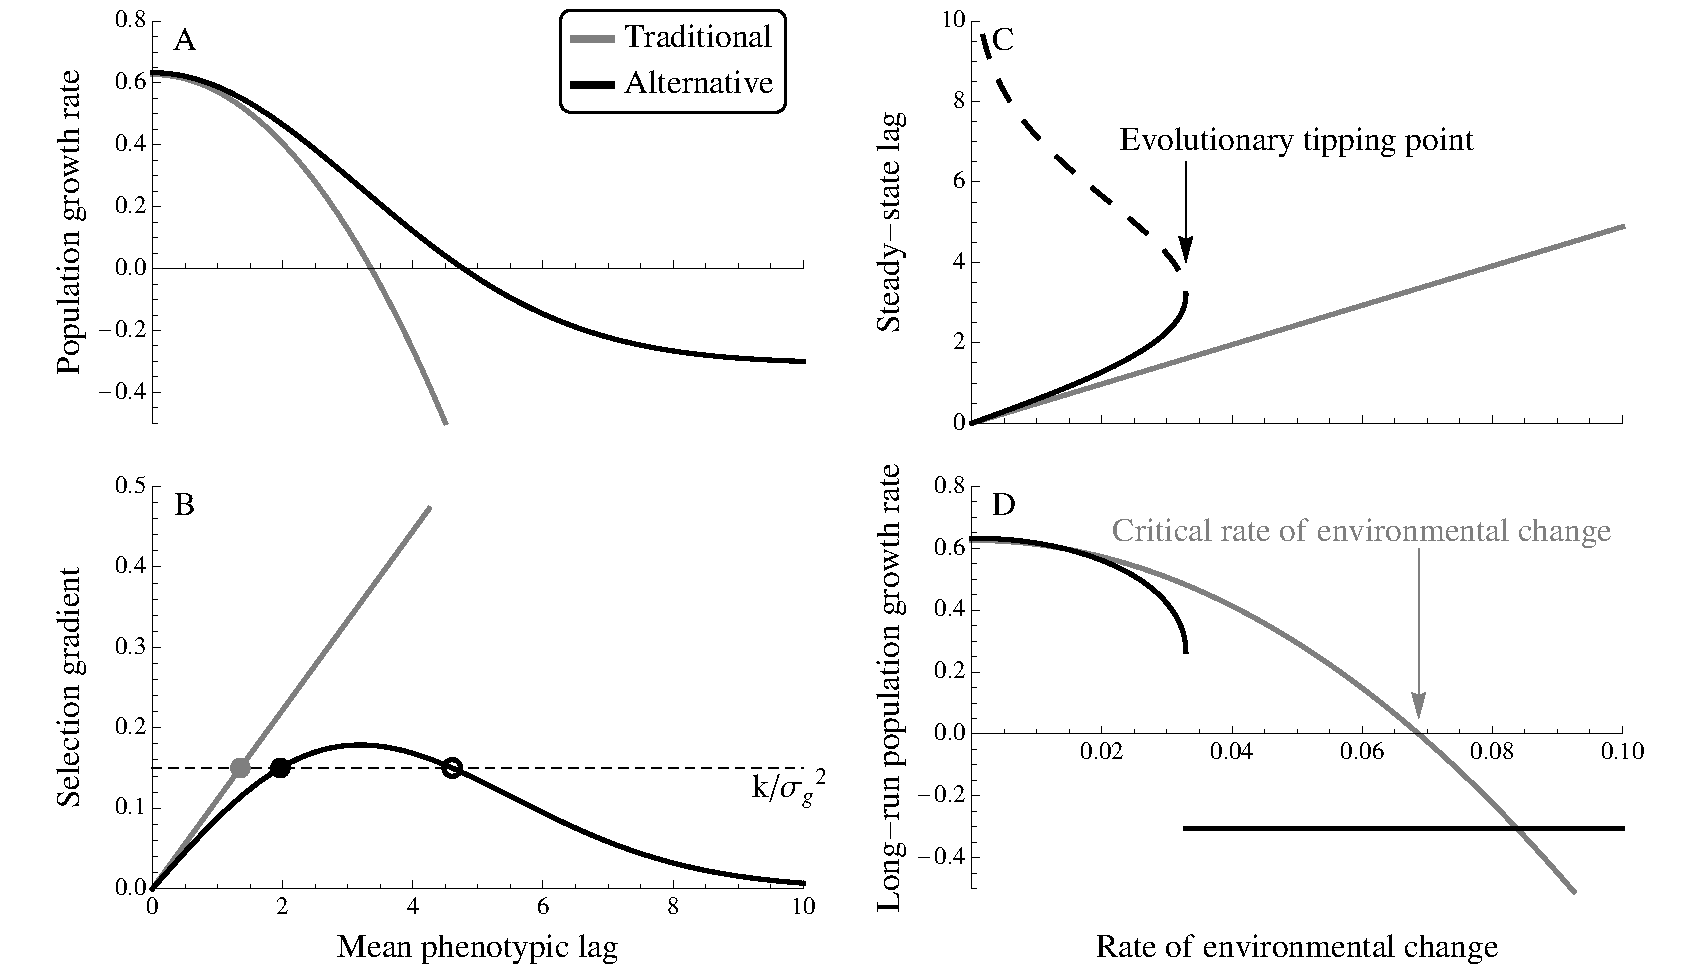
\includegraphics[width=\linewidth]{IMAGES/Didactics}
\caption{
Visual overview of the modelling approach. 
Population mean growth rates, $\bar{r}$, shown in \textbf{A}, are derived by integrating the traditional (\textit{gray}) and alternative (\textit{black}) fitness functions, $r(z)$, over the phenotypic distribution, $p(z)$.
Taking the derivative of mean population growth rate with respect to the mean trait value, $\mathrm{d}\bar{r}/\mathrm{d}\bar{z}$, gives the selection gradients shown in \textbf{B}.
Setting the the rate of evolution equal to the rate of change in the environmental optimum ($\sigma_g^2\mathrm{d}\bar{r}/\mathrm{d}\bar{z} = k$; where the dashed line intersects the solid curves in \textbf{B}) gives the steady-state lags, $\hat{l}$, shown in \textbf{C}.
With the traditional fitness function all steady-state lags are stable (filled circles in \textbf{B} and solid lines in \textbf{C}), while those that are on the decreasing portion of the selection gradient with the alternative fitness function are unstable (open circle in \textbf{B} and dashed lines in \textbf{C}). 
Evaluating population mean growth rate at a stable steady-state lag gives the long-run population growth rates shown in \textbf{D}.
The rate of change that causes a long-run growth rate of zero is the critical rate of environmental change.
Because the long-run population growth rate with an alternative fitness function switches sign without crossing zero at the bifurcation point in \textbf{C}, we call this rate of environmental change an evolutionary tipping point.  
Parameters: $r_m = \log(2)$, $\sigma_w^2 = 9$, $\sigma_e^2 = 1$, $\sigma_g^2\approx0.18$, and $d=1$.
}
\label{SSGrowth}
\end{figure}

\begin{figure}[!ht]
\centering
%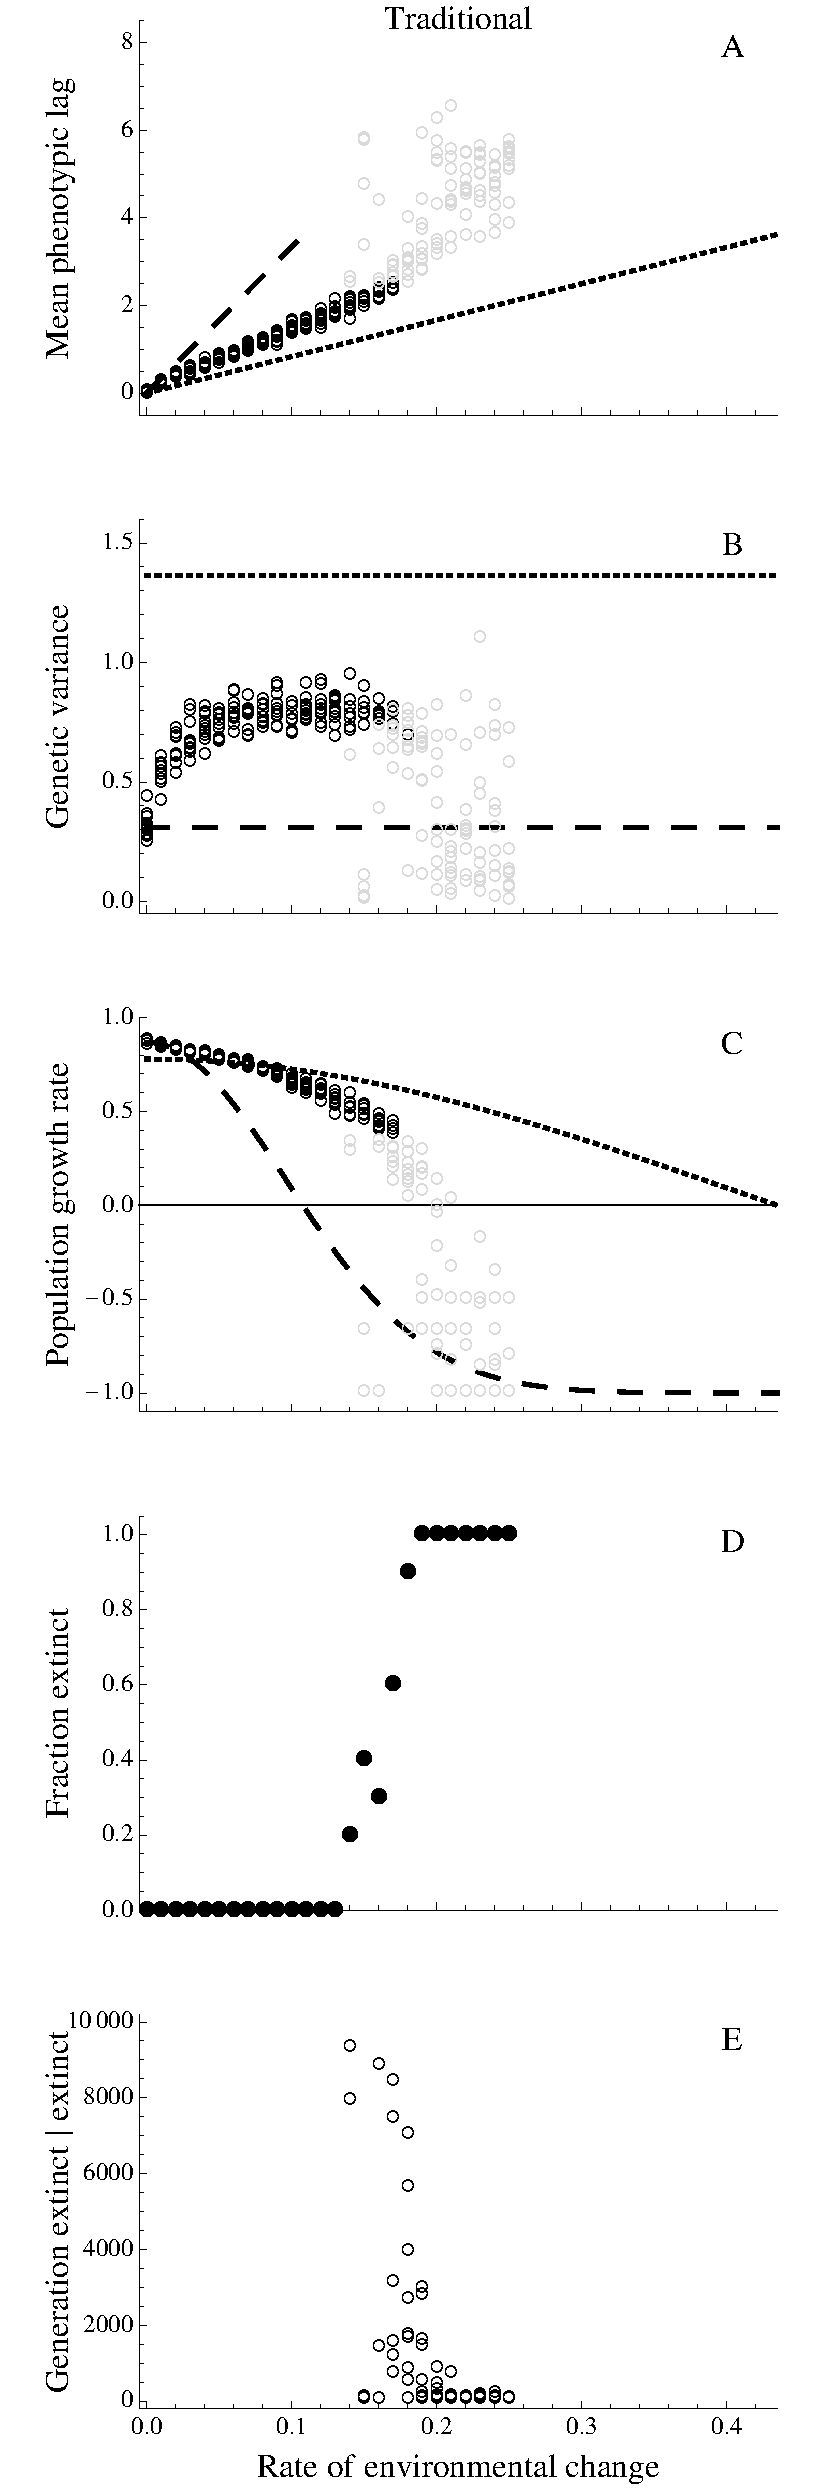
\includegraphics[width=0.45\linewidth]{IMAGES/TradSummaryMeanLargeBurn}
%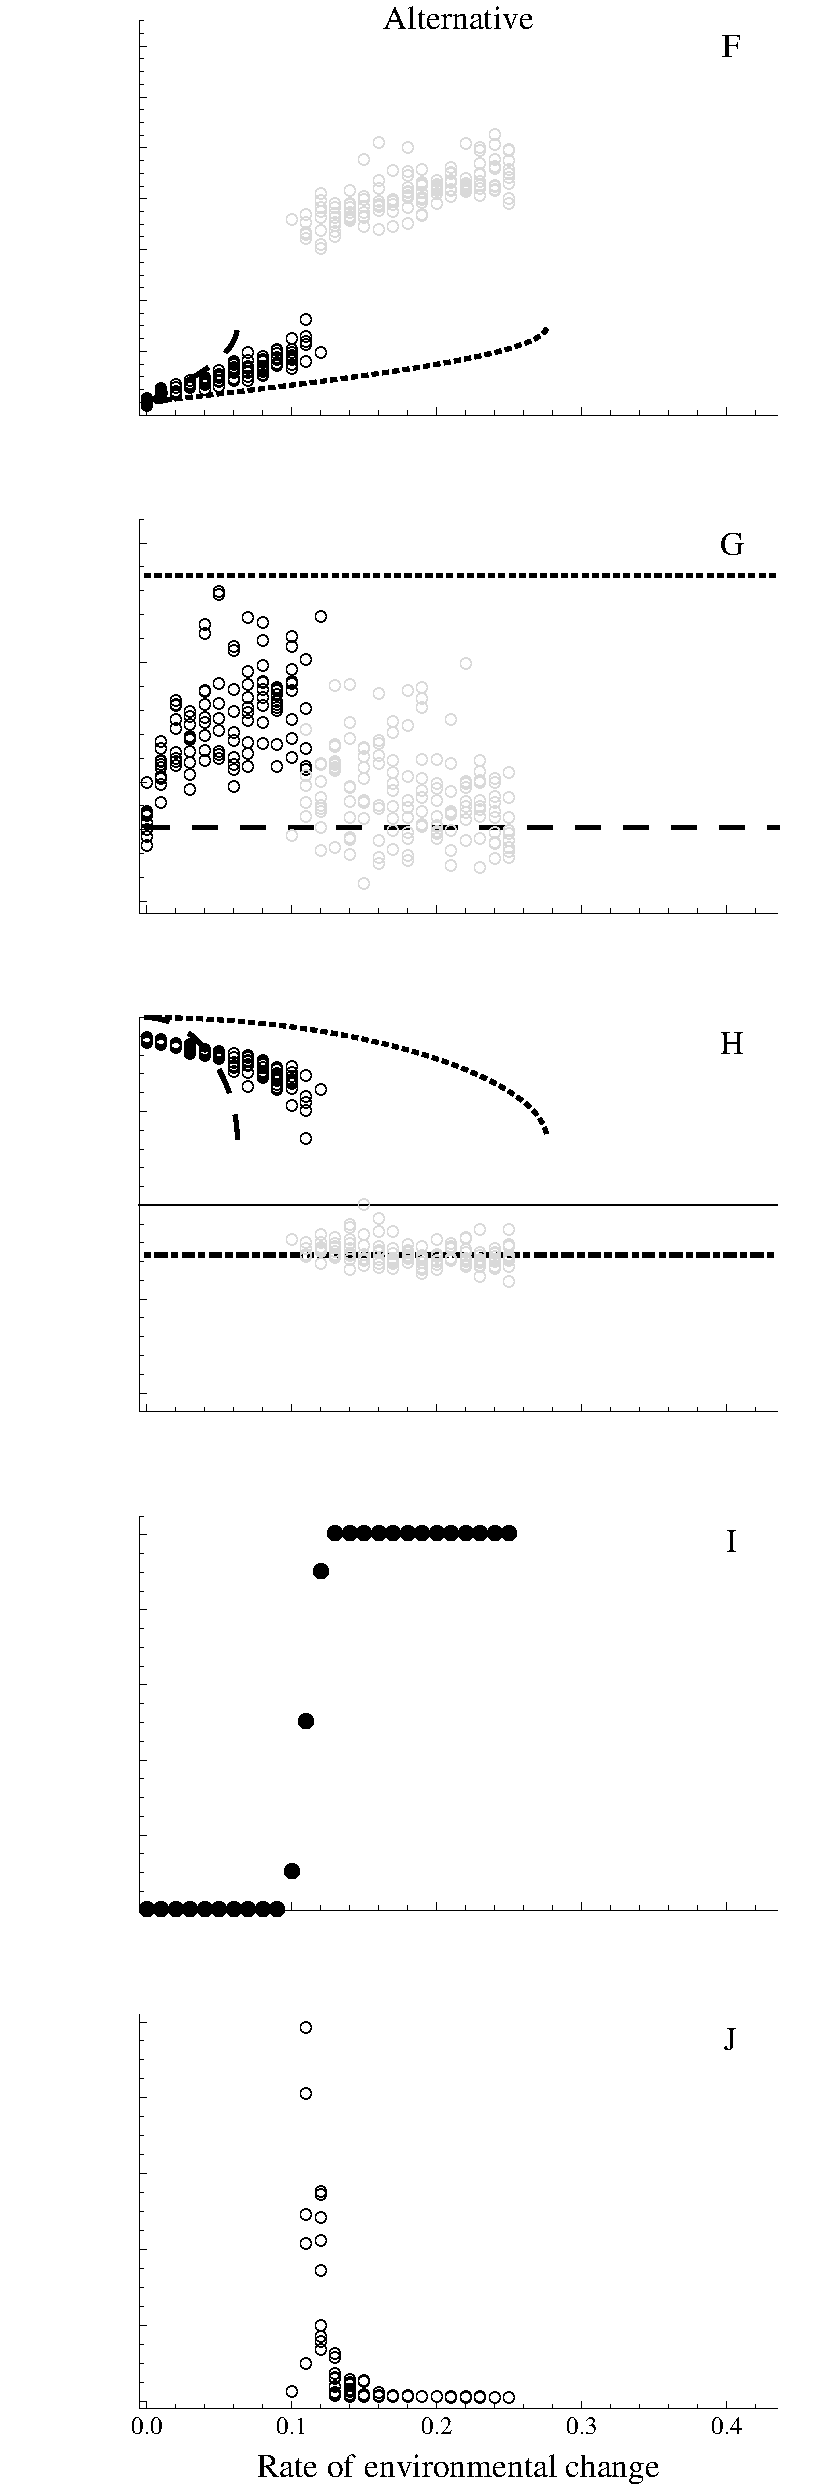
\includegraphics[width=0.45\linewidth]{IMAGES/AltSummaryMeanLargeBurn}
\caption{
Discrete-time, individual-based simulation results with traditional (\textbf{A}-\textbf{E}) and alternative (\textbf{F}-\textbf{J}) fitness functions.
In discrete time the traditional fitness function is $W(z) = \exp\left[ -(\theta - z)^2 / (2\sigma_w^2) \right]$ \citep[][equation 1]{Burger1995} and the alternative fitness function is $W^*(z) = \exp\left[ d(W(z) - 1)\right]$.
``Population growth rate" is the number of offspring surviving viability selection (before density-dependence) divided by the number of parents, minus one. 
``Fraction extinct" is the number of replicates that go extinct before the end of the simulation (generation 11,000).
In \textbf{A}-\textbf{C} and \textbf{F}-\textbf{H}, circles give mean values over the last 10 recorded time points (every 100 generations) for each replicate simulation (10 for each rate of environmental change), or over all recorded time points since the burn-in if less than 10 time points since the burn-in.
Gray circles are replicates that went extinct before the end of the simulation.  
Broken curves in \textbf{A}-\textbf{C}, and \textbf{F}-\textbf{H} give analytic results using the stochastic-house-of-cards (dashed) and neutral (dotted) approximations for genetic variance \citep[equations 14 and 15 in][]{Burger1995}.
Paremeters as in \cite{Burger1995}: $B = 2$, $\sigma_w^2 = 9$, $\sigma_e^2 = 1$, $K=512$, $\mu = 2\times10^{-4}$, $\alpha^2 = 0.05$, $n=50$, and $d=1$.
}
\label{ModerateSummaryLast}
\end{figure}

\begin{figure}[!ht]
\centering
%\includegraphics[width=\linewidth]{IMAGES/EarlyWarningSigns.eps}
\caption{
Generic early-warning signs of tipping points.
Here the rate of environmental change, $k$, gradually increases from 0 by $10^{-6}$ phenotypic units every generation, eventually causing extinction.
With the traditional fitness function (\textbf{A}-\textbf{C}) there is no saddle-node bifurcation and extinction occurs as the rate of environmental change approaches $k=0.175$, as in Figure \ref{ModerateSummaryLast}.
On the other hand, with the alternative fitness function (\textbf{D}-\textbf{F}) there is a saddle-node bifurcation and extinction is caused by an evolutionary tipping point near $k = 0.125$, as in Figure \ref{ModerateSummaryLast}.
Nevertheless, in both cases the temporal variance in mean phenotypic lag (\textit{black}) and population growth rate (\textit{gray}) tend to increase (\textbf{B},\textbf{E}) and Kendall rank correlation coefficients, $\tau$, do not differ significantly between the two fitness functions (\textbf{G}; details in text).
\textbf{C} and \textbf{F} show the dynamics of lag-1 autocorrelation in mean phenotypic lag and population growth rate for both fitness functions, and the Kendall rank correlation coefficients (\textbf{H}) indicate that a consistent increase in the lag-1 autocorrelation of population growth rate may be the best predictor of an approaching evolutionary tipping point for this set of parameters (details in text).
Shown are ten replicate simulations for each fitness function, with parameters as in Figure \ref{ModerateSummaryLast}.
Variance and lag-1 autocorrelation are measured for each replicate separately, using non-intersecting windows of 30 consecutively recorded time points, each 100 generations apart.
}
\label{ModerateWarnings}
\end{figure}

\begin{figure}[!ht]
\centering
%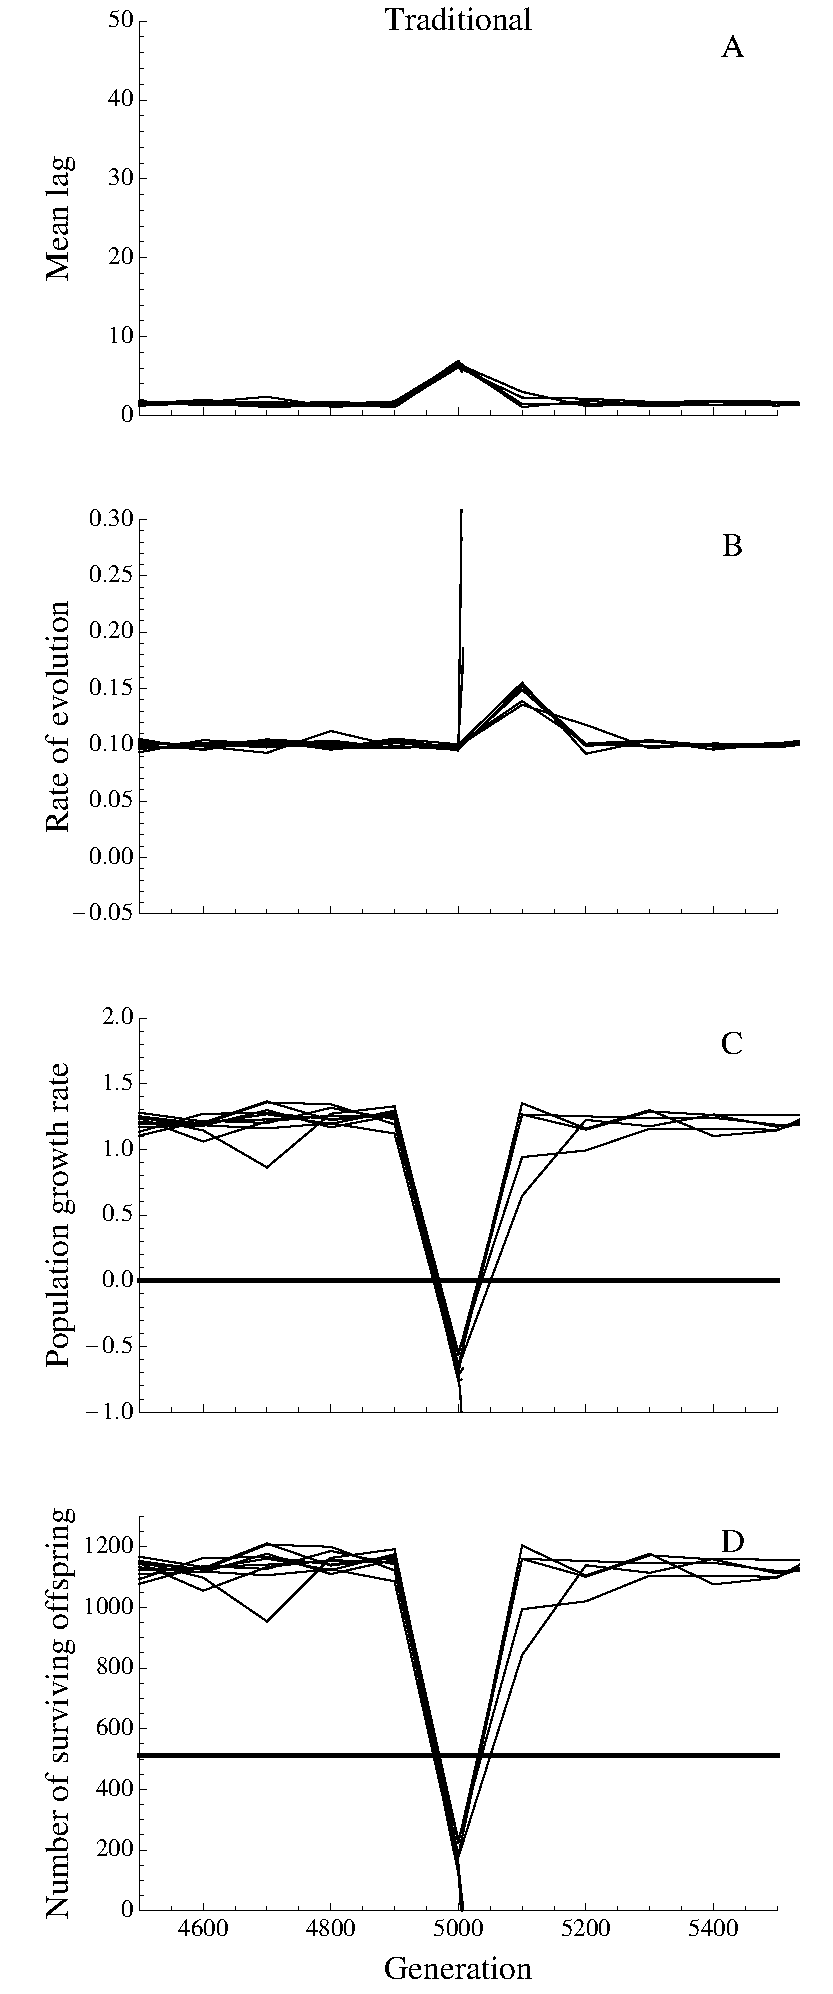
\includegraphics[width=0.45\linewidth]{IMAGES/TradHysteresisSnapshotLarge}
%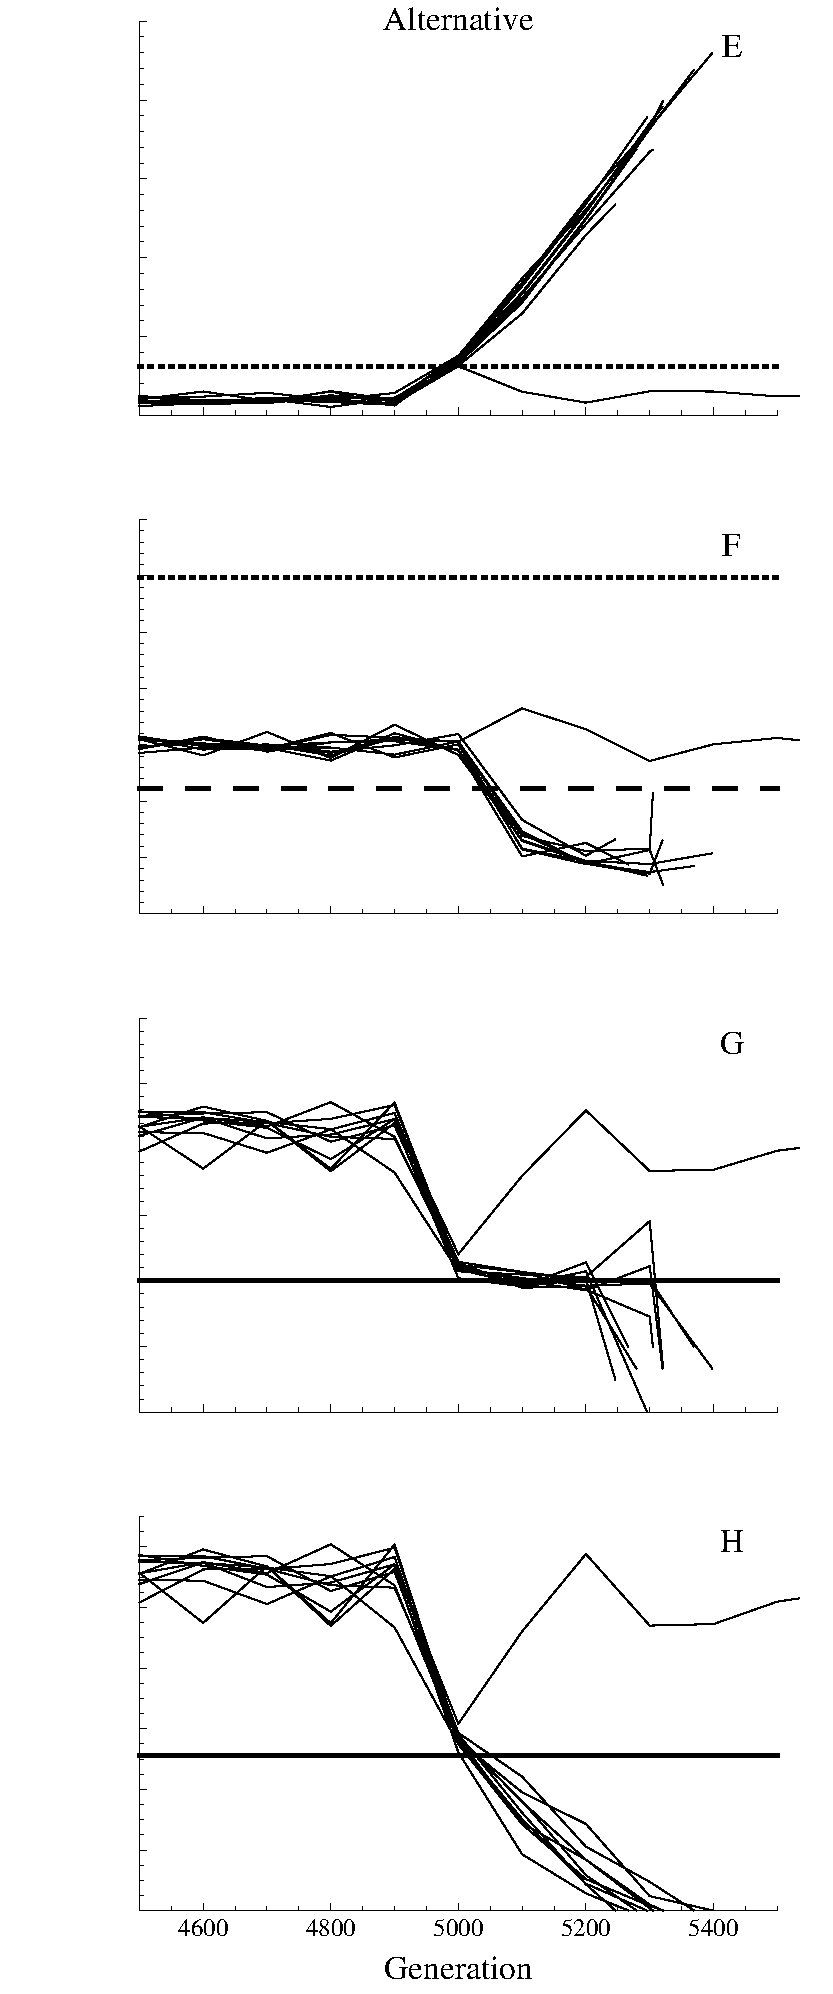
\includegraphics[width=0.45\linewidth]{IMAGES/AltHysteresisSnapshotLarge}
\caption{
Evolutionary hysteresis prevents evolutionary rescue and creates an extinction debt.
Here the optimum trait value increases gradually ($k=0.1$), experiences a sudden jump (5 phenotypic units) at generation 5000, and from there continues to increase at the gradual rate ($k=0.1$).  
With the traditional fitness function (\textbf{A}-\textbf{D}), the sudden increase in mean lag at generation 5000 causes an increase in the strength of selection and hence in the rate of evolution, rescuing populations from extinction.
With the alternative fitness function (\textbf{E}-\textbf{F}), the mean lag increases to values that are often just beyond the basin of attraction of the steady-state lag at $k=0.1$ (dotted line in \textbf{E}, using the neutral approximation for genetic variance; $k=0.1$ is beyond the tipping point with the stochastic-house-of-cards approximation for genetic variance).
(\textbf{F}) The rate of evolution then declines (except in one lucky replicate that does not escape the basin of attraction), causing further increases in the mean lag, which further decreases the rate of evolution, and so on, leading to an apparent existential crisis.
Broken lines show the maximum rate of evolution using the neutral (dotted) and stochastic-house-of-cards (dashed) approximations for genetic variance.
(\textbf{G}) The ever increasing mean lag lowers the population mean growth rate, eventually reaching values below replacement (horizontal line).
(\textbf{H}) This drop in population growth rates ultimately, some $\sim$300 generations later, results in extinction.
The horizontal line is the maximum number of parents, $K$.
Here the fitness functions (see Figure \ref{ModerateSummaryLast}) are multiplied by $(1-d')$, the probability that an optimally adapted individual survives viability selection.
This generalization gives more flexibility in minimum growth rate without affecting the strength of selection.
Parameters as in Figure \ref{ModerateSummaryLast}, except $B=3$ and $d'=0.1$.
}
\label{HysteresisSnapshot}
\end{figure}

\end{document}
